\chapter{Der Simulator}

\section{Die grafische Benutzerschnittstelle}

\begin{figure}[htbp]
	\centering
	\fbox{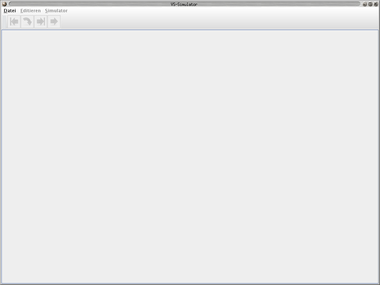
\includegraphics{images/ss-neues-fenster-klein}}
	\caption{Der Simulator nach dem ersten Starten}
	\label{fig:NeuesFenster}
\end{figure}

Der Simulator pr\"{a}sentiert sich nach dem ersten Starten wie in Abbildung \ref{fig:NeuesFenster}. F\"{u}r die Erstellung einer neuen Simulation wird im Men\"{u} ``Datei'' (Abbildung \ref{fig:DateiMenue}) der Punkt ``Neue Simulation'' ausgew\"{a}hlt, wo anschlie�end das Einstellungsfenster f\"{u}r die neue Simulation erscheint.  Auf die einzelnen Optionen wird sp\"{a}ter genauer eingegangen und es werden nun nur die Standardeinstellungen \"{u}bernommen. Die GUI mit einer frischen Simulation sieht dann wie in Abbildung \ref{fig:NeuErstellteSimulation} aus.

\begin{figure}[htbp]
	\centering
	\fbox{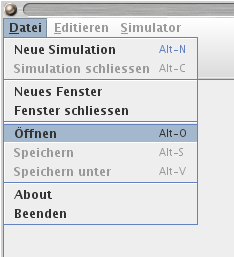
\includegraphics[width=14cm]{images/ss-datei-menu}}
	\caption{Datei-Men\"{u}}
	\label{fig:DateiMenue}
\end{figure}

\subsubsection{Die Men\"{u}zeile}

Im Datei-Men\"{u} (Abbildung \ref{fig:DateiMenue}) lassen sich neue Simulationen erstellen oder die aktuell ge\"{o}ffnete Simulation schliessen. Neue Simulationen \"{o}ffnen sich standardm\"{a}�ig in einem neuen Tab. Es k\"{o}nnen allerdings auch neue Simulationsfenster, die wiederrum eigene Tabs besitzen, ge\"{o}ffnet oder geschlossen werden. In jedem Tab befindet sich eine von den Anderen vollst\"{a}ndig unabh\"{a}ngige Simulation. Es k\"{o}nnen somit beliebig viele Simulationen parallel ausgef\"{u}hrt werden. Die Men\"{u}eintr\"{a}ge ``\"{O}ffnen'', ``Speichern'' und ``Speichern unter'' dienen f\"{u}r das Laden und Speichern von Simulationen. 

\begin{figure}[htbp]
	\centering
	\fbox{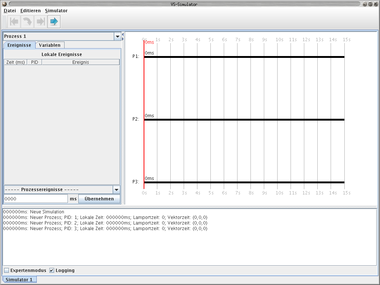
\includegraphics{images/ss-neue-simulation-klein}}
	\caption{Eine neue Simulation}
	\label{fig:NeuErstellteSimulation}
\end{figure}

\"{U}ber das Editieren-Men\"{u} gelangt man zu den Simulationseinstellungen, worauf sp\"{a}ter genauer eingegangen wird. Es werden in diesem Men\"{u} auch alle beteiligten Prozesse zum Editieren aufgelistet. W\"{a}hlt man dort einen Prozess aus, dann \"{o}ffnet sich der dazugeh\"{o}rige Prozesseditor. Auf diesen wird ebenso sp\"{a}ter genauer eingegangen. Das Simulator-Men\"{u} bietet die selben Optionen wie die Toolbar, welche im n\"{a}chsten Teilkapitel beschrieben wird.

Einige Men\"{u}unterpunkte sind erst erreichbar, wenn im aktuellen Fenster bereits eine Simulation erstellt oder geladen wurde.

\subsubsection{Die Toolbar}

Oben links im Simulator befindet sich die Toolbar (Abbildung \ref{fig:Toolbar}). Die Toolbar enth\"{a}lt die Funktionen, die vom Benutzer am h\"{a}ufigsten verwendet werden.

\begin{figure}[htbp]
	\centering
	\fbox{
\includegraphics[width=5cm]{images/ss-neue-simulation-toolbar}}
	\caption{Die Men\"{u}zeile inklusive Toolbar}
	\label{fig:Toolbar}
\end{figure}

Die Toolbar bietet vier verschiedene Funktionalit\"{a}ten an:

\begin{itemize}
	%\setlength{\itemsep}{-1mm}
	\item Starten der Simulation; kann nur bet\"{a}tigt werden, wenn die Simulation derzeit nicht l\"{a}uft.
	\item Pausieren der Simulation, kann nur bet\"{a}tigt werden, wenn die Simulation derzeit l\"{a}uft.
	\item Wiederholen der Simulation, kann nicht bet\"{a}tigt werden, wenn die Simulation noch nicht gestartet wurde. 
	\item Zur\"{u}cksetzen der Simulation, kann nur bet\"{a}tigt werden, wenn die Simulation pausiert wurde oder wenn die Simulation abgelaufen ist.
\end{itemize}

Die Toolbar l\"{a}sst sich auch nach Belieben repositionieren (z.B. links, rechts oder unten des Simulatorfensters). Hierf\"{u}r muss per ``Drag-n-Drop'' die ``raue Fl\"{a}che'' zur Zielposition gezogen werden.

\subsubsection{Die Visualisierung}

\begin{figure}[htbp]
	\centering
	\fbox{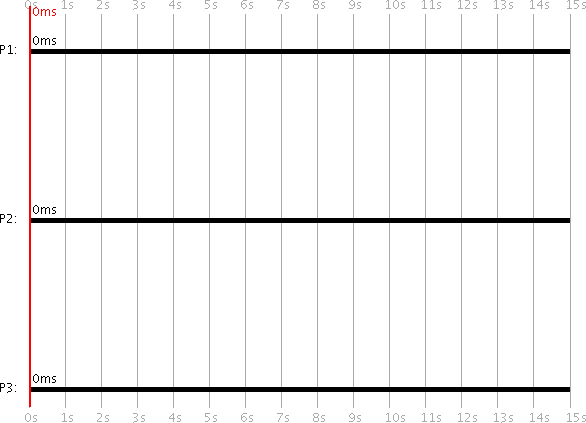
\includegraphics[width=14cm]{images/ss-visualisierung}}
	\caption{Visualisierung einer noch nicht gestarteten Simulation}
	\label{fig:Visualisierung}
\end{figure}

Mittig rechts in Abbildung \ref{fig:NeuErstellteSimulation} befindet sich die grafische Repr\"{a}sentation der Simulation. Die X-Achse gibt die Zeit in Millisekunden an. Unsere Demo-Simulation endet nach genau 15 Sekunden. In Abbildung \ref{fig:Visualisierung} sind 3 Prozesse (mit den PIDs 1, 2 und 3) dargestellt, die jeweils einen eigenen horizontalen schwarzen Balken besitzen. Auf diesen Prozessbalken kann der Benutzer die jeweilige lokale Prozesszeit ablesen. Die vertikale rote Linie stellt die globale Simulationszeit dar. 

Die Prozessbalken dienen auch f\"{u}r Start- und Zielpunkte von Nachrichten. Wenn beispielsweise Prozess 1 eine Nachricht zum Prozess 2 verschickt, so wird eine Linie vom einen Prozessbalken zum Anderen gezeichnet. Nachrichten, die ein Prozess an sich selbst schickt, werden nicht visualisiert. Sie werden aber im Loggfenster (mehr dazu sp\"{a}ter) protokolliert.

Eine andere M\"{o}glichkeit einen Prozesseditor aufzurufen ist ein Linksklick auf den zum Prozess geh\"{o}rigen Prozessbalken. Dies muss also nicht zwingend \"{u}ber das Simulator-Men\"{u} geschehen. Ein Rechtsklick hingegen \"{o}ffnet ein Popup-Fenster mit weiteren Auswahlm\"{o}glichkeiten (Abbildung \ref{fig:RechtsklickProzessbalken}). Ein Prozess kann \"{u}ber das Popup-Men\"{u} nur dann abst\"{u}rzen oder wiederbelebt werden, wenn die Simulation aktuell l\"{a}uft.

\begin{figure}[htbp]
	\centering
	\fbox{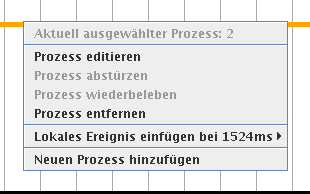
\includegraphics[width=8.8cm]{images/ss-rechtsklick-prozessbalken}}
	\caption{Rechtsklick auf einen Prozessbalken}
	\label{fig:RechtsklickProzessbalken}
\end{figure}

Generell kann die Anzahl der Prozesse nach belieben variieren. Die Dauer der Simulation betr\"{a}gt mindestens 5 -und maximal 120 Sekunden. Die Simulation endet erst, wenn die globale Zeit 15 Sekunden erreicht hat, und nicht, wenn eine lokale Prozesszeit die 15 Sekunden erreicht.

\subsubsection{Farbliche Differenzierung}

Farben helfen dabei die Vorg\"{a}nge einer Simulation zu deuten. Standardm\"{a}�ig werden die Prozesse (Prozessbalken) und Nachrichten mit den Farben wie in Tabelle \ref{tb:Farben} aufgelistet dargestellt. Dies sind lediglich die Standarfarben, welche man \"{u}ber die Einstellungen umkonfigurieren kann.

\begin{table}
	\fbox{
	\begin{tabular}{c|l}
		\textbf{Prozessfarbe} & \textbf{Bedeutung} \\
		\hline 
		 	Schwarz & Simulation l\"{a}uft derzeit nicht (z.B. noch nicht gestartet, abgelaufen oder\\
				& pausiert)\\
		 	Orange & Die Maus befindet sich \"{u}ber den Prozessbalken\\
		 	Rot & Der Prozess ist abgest\"{u}rzt\\
			& \\
		\textbf{Nachrichtfarbe} & \textbf{Bedeutung} \\
		\hline 
		 	Gr\"{u}n & Die Nachricht ist noch unterwegs und hat das Ziel noch nicht erreicht\\
		 	Blau & Die Nachricht hat das Ziel erfolgreich erreicht\\
		 	Rot & Die Nachricht ging verloren (entweder weil der Zielprozess abgest\"{u}rzt ist\\
				& oder weil sie unterwegs verloren ging)\\

	\end{tabular}\\
	}
	\caption{Farbliche Differenzierung von Prozessen und Nachrichten}
	\label{tb:Farben}
\end{table}

\subsubsection{Die Sidebar}

Mithilfe der Sidebar lassen sich Ereignisse von Prozessen verwalten. Ganz oben in Abbildung \ref{fig:Sidebar} ist der zu verwaltende Prozess selektiert (hier mit der PID 1). In dieser Prozessauswahl gibt es auch die M\"{o}glichkeit ``Alle Prozesse'' auszuw\"{a}hlen, womit die Ereignisse aller Prozesse gleichzeitig verwaltet werden k\"{o}nnen. Unter ``Lokale Ereignisse'' versteht man diejenigen Ereignisse, die auftreten, wenn eine bestimmte lokale Zeit des dazugeh\"{o}rigen Prozesses eingetreten ist. Die darunterliegende Ereignistabelle listet alle programmierten Ereignisse (hier noch keine vorhanden) mitsamt Eintrittszeiten sowie den PIDs auf.

\begin{figure}[htbp]
	\centering
	\fbox{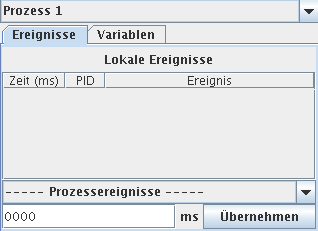
\includegraphics[width=9cm]{images/ss-sidebar}}
	\caption{Die Sidebar mit leerem Ereigniseditor}
	\label{fig:Sidebar}
\end{figure}

F\"{u}r die Erstellung eines neuen Ereignisses kann der Benutzer entweder mit einem Rechtsklick auf einen Prozessbalken (Abbildung \ref{fig:RechtsklickProzessbalken}) klicken, oder unterhalb der Ereignistabelle ein Ereignis ausw\"{a}hlen (Abbildung \ref{fig:Ereignisauswahl}), im darunterliegendem Textfeld die Zeit eintragen und auf ``\"{U}bernehmen'' klicken. Beispielsweise wurden auf Abbildung \ref{fig:SidebarMitEreignissen} drei Ereignisse hinzugef\"{u}gt: Absturz nach 123ms, Wiederbelebung nach 321ms und erneuerter Absturz nach 3000ms des Prozesses mit der ID 1. 

\begin{figure}[htbp]
	\centering
	\fbox{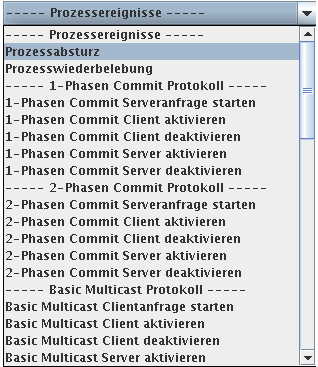
\includegraphics[width=9cm]{images/ss-ereignisauswahl}}
	\caption{Die Ereignisauswahl via Sidebar}
	\label{fig:Ereignisauswahl}
\end{figure}

Mit einem Rechtsklick auf den Ereigniseditor lassen sich alle selektierten Ereignisse entweder kopieren oder l\"{o}schen. Die Eintr\"{a}ge der Spalten f\"{u}r die Zeit und der PID lassen sich nachtr\"{a}glich editieren. Somit besteht eine komfortable M\"{o}glichkeit bereits programmierte Ereignisse auf eine andere Zeit zu verschieben oder einem anderen Prozess zuzuweisen.

In der Sidebar gibt es neben dem Ereignis-Tab einen weiteren Tab ``Variablen''. Hinter diesem Tab verbirgt sich der Prozesseditor des aktuell ausgew\"{a}hlten Prozesses. Dort k\"{o}nnen alle Variablen des Prozesses editiert werden. Dies wird sp\"{a}ter genauer behandelt. 

\begin{figure}[htbp]
	\centering
	\fbox{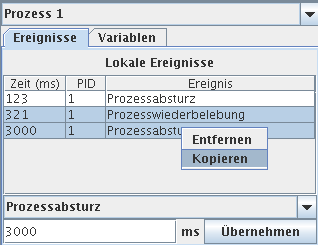
\includegraphics[width=9cm]{images/ss-sidebar-mit-ereignissen}}
	\caption{Der Ereigniseditor mit 3 programmierten Ereignissen}
	\label{fig:SidebarMitEreignissen}
\end{figure}

\subsubsection{Das Loggfenster}

Das Loggfenster (Abbildung \ref{fig:NeuErstellteSimulation}, unten) protokolliert  in chronologischer Reihenfolge alle eingetroffenen Ereignisse. Auf Abbildung \ref{fig:Loggfenster} sieht man das Loggfenster nach Erstellung unserer Simulation, an welcher 3 Prozesse beteiligt sind. Am Anfang eines Loggeintrages wird stets die globale Zeit in Millisekunden protokolliert. Bei jedem Prozess wird ebenso seine lokale Zeit sowie die Lamport- und die Vektor-Zeitstempel aufgef\"{u}hrt. Letztere werden sp\"{a}ter genauer behandelt. 

\begin{figure}[htbp]
	\centering
	\fbox{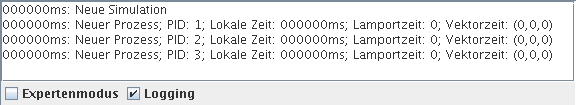
\includegraphics[width=16.5cm]{images/ss-loggfenster}}
	\caption{Das Loggfenster}
	\label{fig:Loggfenster}
\end{figure}

Mit dem Deaktivieren der Checkbox ``Logging'' l\"{a}�t sich das direkte Loggen von Nachrichten tempor\"{a}r deaktivieren. Ohne aktivierter Checkbox erscheinen keine neuen Nachrichten mehr im Loggfenster. Nach Reaktivieren der Checkbox werden alle ausgelassenen Nachrichten nachtr\"{a}glich in das Fenster geschrieben. Eine Deaktivierung des Loggings kann zu verbessertem Leistungsverhalten des Simulators f\"{u}hren (z.B. kein Rucklen; ist vom verwendeten Computer, auf dem der Simulator l\"{a}uft, abh\"{a}ngig). Dieser Umstand ist der sehr langsamen Java-Implementierung der JTextArea-Klasse zu verdanken.

\"{U}ber die Checkbox ``Expertenmodus'' wird der Expertenmodus aktiviert beziehungsweise deaktiviert. 

\section{Der Expertenmodus}

\begin{figure}[htbp]
	\centering
	\fbox{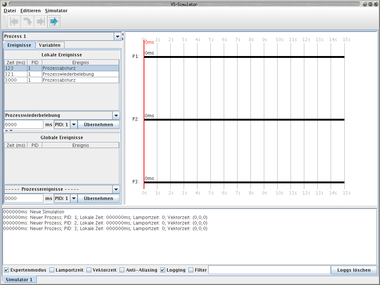
\includegraphics{images/ss-simulation-expertenmodus-klein}}
	\caption{Der Simulator im Expertenmodus}
	\label{fig:SimulationExpertenmodus}
\end{figure}

Der Simulator kann in zwei verschiedenen Modi betrieben werden. Es gibt einen einfachen- und einen Expertenmodus. Der Simulator started standardm\"{a}�ig im einfachen Modus, so dass sich der Benutzer nicht mit der vollen Funktionalit\"{a}t des Simulators auf einmal auseinandersetzen mu�. Der einfache Modus ist \"{u}bersichtlicher, bietet jedoch weniger Funktionen an. Der Expertenmodus eigent sich f\"{u}r mehr erfahrene Anwender und bietet dementsprechend auch mehr Flexibilit\"{a}t. Der Expertenmodus kann \"{u}ber die gleichnamige Checkbox unterhalb des Loggfensters oder \"{u}ber die Simulationseinstellungen aktiviert oder deaktiviert werden.  Auf Abbildung \ref{fig:SimulationExpertenmodus} ist der Simulator im Expertenmodus zu sehen. Wenn man den Simulator im Expertenmodus mit Abbildung \ref{fig:NeuErstellteSimulation} vergleicht, dann fallen einige Unterschiede auf, die nun aufs Weitere behandelt werden.

\begin{figure}[htbp]
	\centering
	\fbox{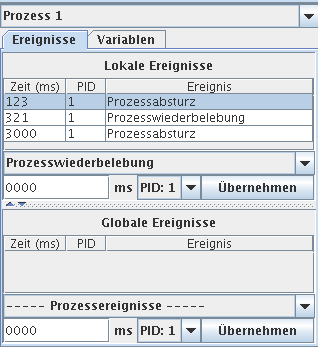
\includegraphics[width=9cm]{images/ss-sidebar-expertenmodus}}
	\caption{Die Sidebar im Expertenmodus}
	\label{fig:SidebarExpertenmodus}
\end{figure}

Der erste Unterschied ist in der Sidebar erkennbar (Abbildung \ref{fig:SidebarExpertenmodus}). Dort sind nun, zus\"{a}tzlich den lokalen Ereignissen, auch globale Ereignisse editierbar.  Wie bereits erw\"{a}hnt, sind unter lokale Ereignisse diejenigen Ereignisse zu verstehen, die auftreten, wenn eine bestimmte lokale Zeit des dazugeh\"{o}rigen Prozesses eingetreten ist. Globale Ereignisse hingegen sind diejenigen Ereignisse, die auftreten, wenn eine bestimmte globale Zeit eingetreten ist. Ein globales Ereignis nimmt die globale Zeit- und ein lokales Ereignis die lokale Prozesszeit als Eintrittskriterium. Globale Ereignisse machen somit nur einen Unterschied, wenn sich die lokalen Prozesszeiten von der globalen Zeit unterscheiden.

Eine weitere neue Funktionalit\"{a}t ist die M\"{o}glichkeit einem neuzuerstellenen Ereignis direkt die PID zuzuweisen. Im einfachen Modus wurde, wenn man ein neues Ereignis erstellte, standardm\"{a}�ig immer die PID des aktuell ausgew\"{a}hlten Prozesses (in der obersten Combo-Box) verwendet. In dieser Combo-Box sollte man gegebenenfalls ``Alle Prozesse'' selektieren, damit im Ereigniseditor stets die Ereignisse aller Prozesse aufgelistet werden.

Weitere Unterschiede machen sich unterhalb des Loggfensters bemerkbar. Dort gibt es unter Anderem zwei neue Checkboxen ``Lamportzeit'' und ``Vektorzeit''.  Aktiviert man eine dieser beiden Checkboxen, dann wird die Lamport- beziehungsweise Vektorzeit in die Visualisierung dargestellt. \"{U}bersichtshalber kann der Benutzer nur jeweils eine dieser beiden Checkboxen aktivieren. Wenn die Lamportzeit-Checkbox bereits aktiviert ist und der Benutzer versucht die Vektorzeit-Checkbox zus\"{a}tzlich zu aktivieren, so wird die Lamportzeit-Checkbox automatisch deaktiviert und virce versa. 

%TODO: Lamport und Vektorzeit definieren!

Die Anti-Aliasing-Checkbox erm\"{o}glicht dem Benutzer Anti-Aliasing zu aktivieren und deaktivieren. Mit aktiviertem Anti-Aliasing werden alle Grafiken der Visualisierung gerundet dargestellt. Aus Performancegr\"{u}nden ist Anti-Aliasing standardm\"{a}�ig deaktiviert.

Je komplexer eine Simulation wird, desto un\"{u}bersichtlicher werden die Eintr\"{a}ge im Loggfenster. Hier f\"{a}llt es zunehmend schwerer die \"{U}bersicht aller Ereignisse zu behalten. Um dem entgegenzuwirken gibt es im Expertenmodus einen Loggfilter, welcher es erm\"{o}glicht nur die wesentlichen Daten aus den Loggs zu filtern. Der Loggfilter wird anhand der dazugeh\"{o}rigen Checkbox ``Filter'' aktiviert beziehungsweise deaktiviert. In der dahinterliegenden Eingabezeile kann ein regul\"{a}rer Ausdruck in Java-Syntax angegeben werden. Beispielsweise werden mit ``\texttt{PID: (1|2)}'' nur Loggzeilen angezeigt, die entweder ``\texttt{PID: 1}'' oder ``\texttt{PID: 2}'' beinhalten. Alle anderen Zeilen, beispielsweise mit ``\texttt{PID: 3}'', werden dabei nicht angezeigt. Mit aktiviertem Loggfilter werden nur die Loggzeilen angezeigt, auf die der regul\"{a}re Ausdruck passt. Der Loggfilter kann auch nachtr\"{a}glich aktiviert werden. Bereits protokollierte Ereignisse werden jedes Mal erneuert gefiltert. Der Loggfilter kann auch w\"{a}hrend einer laufenden Simulation verwendet werden. Wenn der Loggfilter deaktiviert wird, dann werden wieder alle Nachrichten (auch nachtr\"{a}glich) im Loggfenster angezeigt. 

\section{Ereignisse}

Es wird zwischen zwei verschiedenen Haupttypen von Ereignissen unterschieden: Programmierbare Ereignisse und nicht-programmierbare Ereignisse. Programmierbare Ereignisse lassen sich im Ereigniseditor editieren und deren Eintrittszeiten h\"{a}ngen von den lokalen Prozessuhren oder der globalen Uhr ab. Nicht-programmierbare Ereignisse lassen sich hingegen nicht im Ereigniseditor angeben und treten nicht aufgrund einer Uhrzeit auf sondern beispielsweise wenn eine Nachricht eintrifft.

\subsubsection{Prozessabsturz- und Wiederbelebung (programmierbar)}

Die beiden grundliegensten Ereignisse sind ``Prozessabsturz'' sowie ``Prozesswiederbelebung''. Wenn ein Prozess abgest\"{u}rzt ist, so wird sein Prozessbalken in rot dargestellt. Ein abgest\"{u}rzter Prozess kann keine weiteren Ereignisse mehr verarbeiten und, wenn er eine Nachricht empfangen sollte, geht diese verloren. Die einzige Ausnahme bildet ein Wiederbelebungsereignis. Ein abgest\"{u}rzter Prozess kann nichts, ausser wiederbelebt werden. W\"{a}hrend eines Prozessabsturzes l\"{a}uft die lokale Prozessuhr, abgesehen der Lamport- und Vektor-Uhren, wie gewohnt weiter. D.h. es k\"{o}nnte sein, dass ein Prozess einige seiner lokalen Ereignisse gar nicht ausf\"{u}hrt, da er zu den Ereigniseintrittszeiten abgest\"{u}rzt ist. Selbiges trifft nat\"{u}rlich auch auf globale Ereignisse zu. Wenn im echten Leben ein Computer abst\"{u}rzt oder abgeschaltet wird, dann l\"{a}uft dort die Hardwareuhr, unabh\"{a}ngig vom Betriebssystem, auch weiter.

\subsubsection{Aktivierung und Deaktivierung von Protokollen (programmierbar)}

Wir wissen bereits, dass ein Prozess mehrere Protokolle Client- und auch Serverseitig unterst\"{u}tzen kann. Welches Protokoll von einem Prozess unterst\"{u}tzt wird, kann der Benutzer anhand von Protokollaktivierungs- und Protokolldeaktivierungsereignissen konfigurieren. Somit besteht die M\"{o}glichkeit, dass ein gegebener Prozess ein bestimmtes Protokoll erst zu einem bestimmten Zeitpunkt unterst\"{u}tzt und gegebenenfalls ein anderes Protokoll abl\"{o}st. Jedes Protokoll kann entwender Server- oder Clientseitig aktiviert beziehungsweise deaktiviert werden. Welche Protokolle es gibt wird sp\"{a}ter behandelt.

\subsubsection{Weitere Protokollereignisse (programmierbar)}

Der Benutzer hat die Auswahl zwischen f\"{u}nf weiteren Protokollereignissen: 

\begin{itemize}
	\item Aktivierung des Clients des gegebenen Protokolls
	\item Aktivierung des Servers des gegebenen Protokolls
	\item Deaktivierung des Clients des gegebenen Protokolls
	\item Deaktivierung des Servers des gegebenen Protokolls
	\item Starten einer Client/Server-Anfrage des gegebenen Protokolls
\end{itemize}

Ob sich das Ereignis f\"{u}r das Starten einer Anfrage auf den Client oder Server bezieht, h\"{a}ngt vom verwendeten Protokoll ab. Man unterscheidet von Protokollen die Clientseitig- oder Serverseitig eine initiale Anfrage starten. Beispielsweise startet bei dem ``Ping-Pong Protokoll'' der Client- und bei dem ``Commit-Protokollen'' der Server immer die erste Anfrage. Es gibt kein Protokoll, wo Client und Server jeweils eine initiale Anfragen starten k\"{o}nnen. 

Bei allen dieser f\"{u}nf Ereignissen kann der betroffene Prozess noch beliebig andere Dinge, abh\"{a}ngig vom Protokoll, tun. Beispielsweise kann er den Inhalt der Nachricht generieren oder lokale Variablen initialisieren oder eine der lokalen Uhzeiten \"{a}ndern oder Wecker f\"{u}r ``Callback Ereignisse'' setzen (mehr dazu sp\"{a}ter).

\subsubsection{Nachrichtenempfang sowie Antwortnachrichten (nicht-programmierbar)}

Nachdem ein Prozess eine Anfragenachricht versendet hat, und ein weiterer Prozess diese Nachricht erh\"{a}lt, so \"{u}berpr\"{u}ft der Empf\"{a}ngerprozess zun\"{a}chst ob er das dazugeh\"{o}rige Protokoll versteht. Wenn es sich um eine Clientnachricht handelt, so mu� der Empf\"{a}nger ein Server sein und virce versa. Passt alles, so f\"{u}hrt der Empf\"{a}ngerprozess die vom Protokoll definierten Aktionen aus. In der Regel berechnet der Prozess einen Wert und schickt eine Antwortnachricht zur\"{u}ck. Es k\"{o}nnen aber auch beliebig andere Aktionen ausgef\"{u}hrt werden. 

\subsubsection{Callback-Ereignisse (nicht-programmierbar)}

Ein Callback-Ereignis kann von einem Protokoll ausgel\"{o}st werden. Das Protokoll setzt einen Wecker zur welcher lokalen Uhrzeit eine weitere Aktion ausgef\"{u}hrt werden soll. Zum Beispiel lassen sich hiermit Timeouts realisieren, wenn ein Protokoll eine Antwort erwartet, diese aber nicht eintrifft. Nach dem Timeout kann dann eine Anfrage erneuert verschickt werden! Es k\"{o}nnen beliebig viele Callback-Ereignisse definiert werden. Wenn sie noch nicht ausgef\"{u}hrt wurden und aufgrund eines anderen Ereignisses nicht mehr ben\"{o}tigt werden, k\"{o}nnen sie vom Protokoll auch wieder entfernt werden. Wenn ein Callback-Ereignis ausgef\"{u}hrt wird, kann es sich selbst wieder f\"{u}r eine weitere Ausf\"{u}hrung erneuert planen. So lassen sich periodisch wiedereintreffende Ereignisse realisieren. Beispielsweise verwendet das ``Reliable Multicast Protokoll'' Callback-Ereignisse, indem solange Anfragen verschickt werden, bis alle ben\"{o}tigten Antworten vorliegen.

\section{Protokolle}

Im Folgenden werden alle bisher verf\"{u}gbaren Protokolle behandelt. Wie bereits beschrieben wird bei Protokollen zwischen Server- und Clientseite unterschieden. Server k\"{o}nnen auf Clientnachrichten, und Client auf Servernachrichten antworten. Jeder Prozess kann beliebig viele Protokolle sowohl Clientseitig als auch Serverseitig untest\"{u}tzen. Theoretisch ist es auch m\"{o}glich, dass ein Prozess f\"{u}r ein bestimmtes Protokoll gleichzeitig Server und Client ist. Der Benutzer kann auch weitere eigene Protokolle in der Programmiersprache Java mittels einer speziellen API (Application Programming Interface) erstellen. Wie eigene Protokolle erstellt werden k\"{o}nnen wird sp\"{a}ter behandelt. 

\subsection{Beispiel (Dummy) Protokoll}

Das Dummy-Protokoll dient lediglich als leeres Template f\"{u}r die Erstellung eigener Protokolle. Bei der Verwendung des Dummy-Protokolls werden bei Ereignissen lediglich Loggnachrichten ausgegeben, jedoch keine weiteren Aktionen ausgef\"{u}hrt.

\subsection{Das Ping-Pong Protokoll}

\begin{figure}[htbp]
	\centering
	\fbox{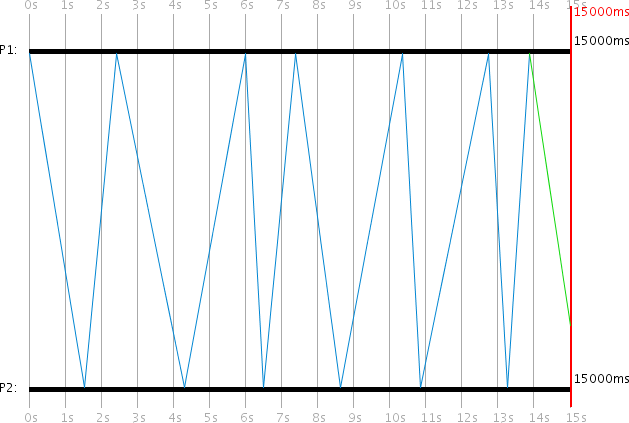
\includegraphics[width=10cm]{images/ss-protokoll-ping-pong}}
	\caption{Das Ping-Pong Protokoll}
	\label{fig:PingPongProto}
\end{figure}

Bei dem Ping-Pong Protokoll (Abbildung \ref{fig:PingPongProto}) werden zwischen zwei Prozessen, Client P1 und Server P2, st\"{a}ndig Nachrichten hin- und hergeschickt. Der Ping-Pong Client startet die erste Anfrage, worauf der Server dem Client antwortet. Auf diese Antwort wird vom Client wiederum geantwortet und so weiter. Jeder Nachricht wird ein Z\"{a}hler mitgeschickt, der bei jeder Station um eins inkrementiert- und jeweils im Loggfenster protokolliert wird. In der Simulation werden erst keine Antwortnachrichten mehr verschickt, wenn entweder eine Nachricht verloren geht, oder wenn die Simulationszeit das Ende erreicht hat. In Tabelle \ref{tb:PingPongTasks} sind alle f\"{u}r dieses Beispiel programmierten Ereignisse aufgef\"{u}hrt! Wichtig ist, dass Prozess 1 seinen Ping-Pong Client aktiviert, bevor er eine Ping-Pong Clientanfrage startet! Wenn die Eintrittszeiten f\"{u}r Aktivierung und das Starten der Anfrage identisch sind, so ordnet der Ereigniseditor diese Ereignisse automatisch in der richtigen Reihenfolge an.  Anhand diesen Beispiels ist auch erkennbar, dass die noch nicht ausgelieferte Nachrichten noch g\"{u}n eingef\"{a}rbt ist. Alle ausgelieferten Nachrichten tragen schon die Farbe Blau.

\begin{table}
	\centering
	\fbox{
	\begin{tabular}{c|c|l}
		\textbf{Zeit (ms)} & \textbf{PID} & \textbf{Ereignis} \\
		\hline 
		 	0 & 1 & Ping Pong Client aktivieren\\
		 	0 & 2 & Ping Pong Server aktivieren\\
		 	0 & 1 & Ping Pong Clientanfrage starten
	\end{tabular}
	}
	\caption{Programmierte Ping-Pong Ereignisse}
	\label{tb:PingPongTasks}
\end{table}

\begin{figure}[htbp]
	\centering
	\fbox{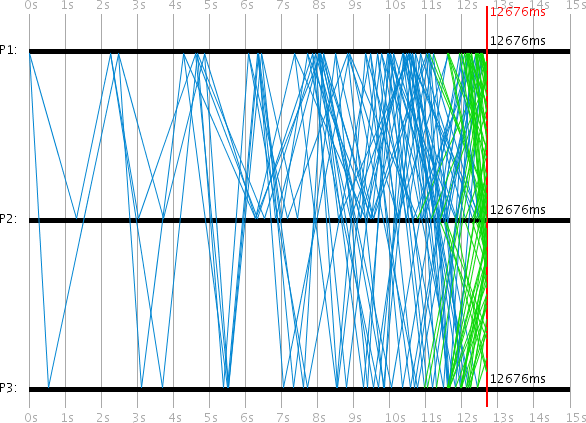
\includegraphics[width=10cm]{images/ss-protokoll-ping-pong-sturm}}
	\caption{Das Ping-Pong Protokoll (Sturm)}
	\label{fig:PingPongSturmProto}
\end{figure}

\"{A}ndert man die Ereignisse wie in Tabelle \ref{tb:PingPongSturmTasks} ab, so l\"{a}sst sich ein Ping-Pong Sturm realisieren. Dort wurde ein neuer Prozess 3 eingef\"{u}hrt, der als Ping-Pong Server fungiert. Als Ursache verdoppelt sich die Anzahl der kursierenden Nachrichten bei jedem Client-Server Roundtrip, da auf jede Clientnachricht stets 2 Serverantworten verschickt werden. In Abbildung \ref{fig:PingPongSturmProto} ist der resultierende Simulationsverlauf dargestellt.

\begin{table}
	\centering
	\fbox{
	\begin{tabular}{c|c|l}
		\textbf{Zeit (ms)} & \textbf{PID} & \textbf{Ereignis} \\
		\hline 
		 	0 & 1 & Ping Pong Client aktivieren\\
		 	0 & 2 & Ping Pong Server aktivieren\\
		 	0 & 3 & Ping Pong Server aktivieren\\
		 	0 & 1 & Ping Pong Clientanfrage starten
	\end{tabular}
	}
	\caption{Programmierte Ping-Pong Ereignisse (Sturm)}
	\label{tb:PingPongSturmTasks}
\end{table}


\subsection{Das Broadcast-Sturm Protokoll}

\begin{figure}[htbp]
	\centering
	\fbox{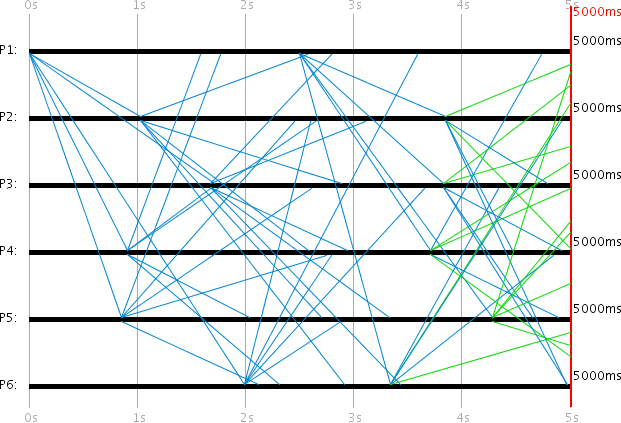
\includegraphics[width=10cm]{images/ss-protokoll-broadcast-sturm}}
	\caption{Das Broadcast-Sturm Protokoll}
	\label{fig:BroadcastSturmProto}
\end{figure}

Das Broadcast-Sturm Protokoll verh\"{a}lt sich \"{a}hnlich wie das Ping-Pong Protokoll. Der Unterschied besteht darin, dass sich das Protokoll anhand einer eindeutigen Broadcast-ID merkt, welche Nachrichten bereits verschickt wurden. Das Broadcast-Sturm Protokoll (Server- und Clientseitig) verschickt alle erhaltenen Nachrichten, sofern sie vom jeweiligen Prozess noch nicht schoneinmal verschickt wurden, erneuert. Somit l\"{a}sst sich, unter Verwendung mehrerer Prozesse (hier 6), wie auf Abbildung \ref{fig:BroadcastSturmProto}, ein Broadcast-Sturm erzeugen. P1 ist der Client und startet je eine Anfrage nach 0ms und 2500ms. Die Simulationsdauer betr\"{a}gt hier genau 5000ms. Da Client nur Servernachrichten und Server nur Clientnachrichten empfangen k\"{o}nnen, ist in dieser Simulation jeder Prozess, wie in Tabelle \ref{tb:BroadcastSturmTasks} angegeben, gleichzeitig Server und Client. 

\begin{table}
	\centering
	\fbox{
	\begin{tabular}{c|c|l}
		\textbf{Zeit (ms)} & \textbf{PID} & \textbf{Ereignis} \\
		\hline 
		 	0000 & 1 & Broadcaststurn Client aktivieren\\
		 	0000 & 2 & Broadcaststurn Client aktivieren\\
		 	0000 & 3 & Broadcaststurn Client aktivieren\\
		 	0000 & 4 & Broadcaststurn Client aktivieren\\
		 	0000 & 5 & Broadcaststurn Client aktivieren\\
		 	0000 & 6 & Broadcaststurn Client aktivieren\\
		 	0000 & 1 & Broadcaststurn Server aktivieren\\
		 	0000 & 2 & Broadcaststurn Server aktivieren\\
		 	0000 & 3 & Broadcaststurn Server aktivieren\\
		 	0000 & 4 & Broadcaststurn Server aktivieren\\
		 	0000 & 5 & Broadcaststurn Server aktivieren\\
		 	0000 & 6 & Broadcaststurn Server aktivieren\\
		 	0000 & 1 & Broadcaststurn Clientanfrage starten\\
		 	2500 & 1 & Broadcaststurn Clientanfrage starten
	\end{tabular}
	}
	\caption{Programmierte Broadcast-Sturm Ereignisse}
	\label{tb:BroadcastSturmTasks}
\end{table}



\subsection{Das Protokoll zur internen Synchronisierung in einem synchronen System}

\subsection{Christians Methode zur externen Synchronisierung}
 lsdkfjds lfjds flsjfsljsd flsdjf sldkfjsdlfkj 
 lsdkfjds lfjds flsjfsljsd flsdjf sldkfjsdlfkj 
 lsdkfjds lfjds flsjfsljsd flsdjf sldkfjsdlfkj 
 lsdkfjds lfjds flsjfsljsd flsdjf sldkfjsdlfkj 
 lsdkfjds lfjds flsjfsljsd flsdjf sldkfjsdlfkj 
 lsdkfjds lfjds flsjfsljsd flsdjf sldkfjsdlfkj 
 lsdkfjds lfjds flsjfsljsd flsdjf sldkfjsdlfkj 
 lsdkfjds lfjds flsjfsljsd flsdjf sldkfjsdlfkj 
 lsdkfjds lfjds flsjfsljsd flsdjf sldkfjsdlfkj 
 lsdkfjds lfjds flsjfsljsd flsdjf sldkfjsdlfkj 
 lsdkfjds lfjds flsjfsljsd flsdjf sldkfjsdlfkj 
 lsdkfjds lfjds flsjfsljsd flsdjf sldkfjsdlfkj 
 lsdkfjds lfjds flsjfsljsd flsdjf sldkfjsdlfkj 
 lsdkfjds lfjds flsjfsljsd flsdjf sldkfjsdlfkj 
 lsdkfjds lfjds flsjfsljsd flsdjf sldkfjsdlfkj 
 lsdkfjds lfjds flsjfsljsd flsdjf sldkfjsdlfkj 
 lsdkfjds lfjds flsjfsljsd flsdjf sldkfjsdlfkj 
 lsdkfjds lfjds flsjfsljsd flsdjf sldkfjsdlfkj 
 lsdkfjds lfjds flsjfsljsd flsdjf sldkfjsdlfkj 
 lsdkfjds lfjds flsjfsljsd flsdjf sldkfjsdlfkj 
 lsdkfjds lfjds flsjfsljsd flsdjf sldkfjsdlfkj 
 lsdkfjds lfjds flsjfsljsd flsdjf sldkfjsdlfkj 
 lsdkfjds lfjds flsjfsljsd flsdjf sldkfjsdlfkj 
 lsdkfjds lfjds flsjfsljsd flsdjf sldkfjsdlfkj 
 lsdkfjds lfjds flsjfsljsd flsdjf sldkfjsdlfkj 
 lsdkfjds lfjds flsjfsljsd flsdjf sldkfjsdlfkj 
 lsdkfjds lfjds flsjfsljsd flsdjf sldkfjsdlfkj 
 lsdkfjds lfjds flsjfsljsd flsdjf sldkfjsdlfkj 
 lsdkfjds lfjds flsjfsljsd flsdjf sldkfjsdlfkj 
 lsdkfjds lfjds flsjfsljsd flsdjf sldkfjsdlfkj 
 lsdkfjds lfjds flsjfsljsd flsdjf sldkfjsdlfkj 
 lsdkfjds lfjds flsjfsljsd flsdjf sldkfjsdlfkj 
 lsdkfjds lfjds flsjfsljsd flsdjf sldkfjsdlfkj 
 lsdkfjds lfjds flsjfsljsd flsdjf sldkfjsdlfkj 
 lsdkfjds lfjds flsjfsljsd flsdjf sldkfjsdlfkj 
 lsdkfjds lfjds flsjfsljsd flsdjf sldkfjsdlfkj 
 lsdkfjds lfjds flsjfsljsd flsdjf sldkfjsdlfkj 
 lsdkfjds lfjds flsjfsljsd flsdjf sldkfjsdlfkj 
 lsdkfjds lfjds flsjfsljsd flsdjf sldkfjsdlfkj 
 lsdkfjds lfjds flsjfsljsd flsdjf sldkfjsdlfkj 
 lsdkfjds lfjds flsjfsljsd flsdjf sldkfjsdlfkj 
 lsdkfjds lfjds flsjfsljsd flsdjf sldkfjsdlfkj 
 lsdkfjds lfjds flsjfsljsd flsdjf sldkfjsdlfkj 
 lsdkfjds lfjds flsjfsljsd flsdjf sldkfjsdlfkj 
 lsdkfjds lfjds flsjfsljsd flsdjf sldkfjsdlfkj 
 lsdkfjds lfjds flsjfsljsd flsdjf sldkfjsdlfkj 
 lsdkfjds lfjds flsjfsljsd flsdjf sldkfjsdlfkj 
 lsdkfjds lfjds flsjfsljsd flsdjf sldkfjsdlfkj 
 lsdkfjds lfjds flsjfsljsd flsdjf sldkfjsdlfkj 
 lsdkfjds lfjds flsjfsljsd flsdjf sldkfjsdlfkj 
 lsdkfjds lfjds flsjfsljsd flsdjf sldkfjsdlfkj 
 lsdkfjds lfjds flsjfsljsd flsdjf sldkfjsdlfkj 
 lsdkfjds lfjds flsjfsljsd flsdjf sldkfjsdlfkj 
 lsdkfjds lfjds flsjfsljsd flsdjf sldkfjsdlfkj 
 lsdkfjds lfjds flsjfsljsd flsdjf sldkfjsdlfkj 
 lsdkfjds lfjds flsjfsljsd flsdjf sldkfjsdlfkj 
 lsdkfjds lfjds flsjfsljsd flsdjf sldkfjsdlfkj 
 lsdkfjds lfjds flsjfsljsd flsdjf sldkfjsdlfkj 
 lsdkfjds lfjds flsjfsljsd flsdjf sldkfjsdlfkj 
 lsdkfjds lfjds flsjfsljsd flsdjf sldkfjsdlfkj 
 lsdkfjds lfjds flsjfsljsd flsdjf sldkfjsdlfkj 
 lsdkfjds lfjds flsjfsljsd flsdjf sldkfjsdlfkj 
 lsdkfjds lfjds flsjfsljsd flsdjf sldkfjsdlfkj 
 lsdkfjds lfjds flsjfsljsd flsdjf sldkfjsdlfkj 
 lsdkfjds lfjds flsjfsljsd flsdjf sldkfjsdlfkj 
 lsdkfjds lfjds flsjfsljsd flsdjf sldkfjsdlfkj 
 lsdkfjds lfjds flsjfsljsd flsdjf sldkfjsdlfkj 
 lsdkfjds lfjds flsjfsljsd flsdjf sldkfjsdlfkj 
 lsdkfjds lfjds flsjfsljsd flsdjf sldkfjsdlfkj 
 lsdkfjds lfjds flsjfsljsd flsdjf sldkfjsdlfkj 
 lsdkfjds lfjds flsjfsljsd flsdjf sldkfjsdlfkj 
 lsdkfjds lfjds flsjfsljsd flsdjf sldkfjsdlfkj 
 lsdkfjds lfjds flsjfsljsd flsdjf sldkfjsdlfkj 
 lsdkfjds lfjds flsjfsljsd flsdjf sldkfjsdlfkj 
 lsdkfjds lfjds flsjfsljsd flsdjf sldkfjsdlfkj 
 lsdkfjds lfjds flsjfsljsd flsdjf sldkfjsdlfkj 
 lsdkfjds lfjds flsjfsljsd flsdjf sldkfjsdlfkj 
 lsdkfjds lfjds flsjfsljsd flsdjf sldkfjsdlfkj 
 lsdkfjds lfjds flsjfsljsd flsdjf sldkfjsdlfkj 
 lsdkfjds lfjds flsjfsljsd flsdjf sldkfjsdlfkj 
 lsdkfjds lfjds flsjfsljsd flsdjf sldkfjsdlfkj 
 lsdkfjds lfjds flsjfsljsd flsdjf sldkfjsdlfkj 
 lsdkfjds lfjds flsjfsljsd flsdjf sldkfjsdlfkj 
 lsdkfjds lfjds flsjfsljsd flsdjf sldkfjsdlfkj 
 lsdkfjds lfjds flsjfsljsd flsdjf sldkfjsdlfkj 
 lsdkfjds lfjds flsjfsljsd flsdjf sldkfjsdlfkj 
 lsdkfjds lfjds flsjfsljsd flsdjf sldkfjsdlfkj 
 lsdkfjds lfjds flsjfsljsd flsdjf sldkfjsdlfkj 
 lsdkfjds lfjds flsjfsljsd flsdjf sldkfjsdlfkj 
 lsdkfjds lfjds flsjfsljsd flsdjf sldkfjsdlfkj 
 lsdkfjds lfjds flsjfsljsd flsdjf sldkfjsdlfkj 
 lsdkfjds lfjds flsjfsljsd flsdjf sldkfjsdlfkj 
 lsdkfjds lfjds flsjfsljsd flsdjf sldkfjsdlfkj 
 lsdkfjds lfjds flsjfsljsd flsdjf sldkfjsdlfkj 
 lsdkfjds lfjds flsjfsljsd flsdjf sldkfjsdlfkj 
 lsdkfjds lfjds flsjfsljsd flsdjf sldkfjsdlfkj 
 lsdkfjds lfjds flsjfsljsd flsdjf sldkfjsdlfkj 
 lsdkfjds lfjds flsjfsljsd flsdjf sldkfjsdlfkj 
 lsdkfjds lfjds flsjfsljsd flsdjf sldkfjsdlfkj 
 lsdkfjds lfjds flsjfsljsd flsdjf sldkfjsdlfkj 
 lsdkfjds lfjds flsjfsljsd flsdjf sldkfjsdlfkj 
 lsdkfjds lfjds flsjfsljsd flsdjf sldkfjsdlfkj 
 lsdkfjds lfjds flsjfsljsd flsdjf sldkfjsdlfkj 
 lsdkfjds lfjds flsjfsljsd flsdjf sldkfjsdlfkj 
 lsdkfjds lfjds flsjfsljsd flsdjf sldkfjsdlfkj 
 lsdkfjds lfjds flsjfsljsd flsdjf sldkfjsdlfkj 
 lsdkfjds lfjds flsjfsljsd flsdjf sldkfjsdlfkj 
 lsdkfjds lfjds flsjfsljsd flsdjf sldkfjsdlfkj 
 lsdkfjds lfjds flsjfsljsd flsdjf sldkfjsdlfkj 
 lsdkfjds lfjds flsjfsljsd flsdjf sldkfjsdlfkj 
 lsdkfjds lfjds flsjfsljsd flsdjf sldkfjsdlfkj 
 lsdkfjds lfjds flsjfsljsd flsdjf sldkfjsdlfkj 
 lsdkfjds lfjds flsjfsljsd flsdjf sldkfjsdlfkj 
 lsdkfjds lfjds flsjfsljsd flsdjf sldkfjsdlfkj 
 lsdkfjds lfjds flsjfsljsd flsdjf sldkfjsdlfkj 
 lsdkfjds lfjds flsjfsljsd flsdjf sldkfjsdlfkj 
 lsdkfjds lfjds flsjfsljsd flsdjf sldkfjsdlfkj 
 lsdkfjds lfjds flsjfsljsd flsdjf sldkfjsdlfkj 
 lsdkfjds lfjds flsjfsljsd flsdjf sldkfjsdlfkj 
 lsdkfjds lfjds flsjfsljsd flsdjf sldkfjsdlfkj 
 lsdkfjds lfjds flsjfsljsd flsdjf sldkfjsdlfkj 
 lsdkfjds lfjds flsjfsljsd flsdjf sldkfjsdlfkj 
 lsdkfjds lfjds flsjfsljsd flsdjf sldkfjsdlfkj 
 lsdkfjds lfjds flsjfsljsd flsdjf sldkfjsdlfkj 
 lsdkfjds lfjds flsjfsljsd flsdjf sldkfjsdlfkj 
 lsdkfjds lfjds flsjfsljsd flsdjf sldkfjsdlfkj 
 lsdkfjds lfjds flsjfsljsd flsdjf sldkfjsdlfkj 
 lsdkfjds lfjds flsjfsljsd flsdjf sldkfjsdlfkj 
 lsdkfjds lfjds flsjfsljsd flsdjf sldkfjsdlfkj 
 lsdkfjds lfjds flsjfsljsd flsdjf sldkfjsdlfkj 
 lsdkfjds lfjds flsjfsljsd flsdjf sldkfjsdlfkj 
 lsdkfjds lfjds flsjfsljsd flsdjf sldkfjsdlfkj 
 lsdkfjds lfjds flsjfsljsd flsdjf sldkfjsdlfkj 
 lsdkfjds lfjds flsjfsljsd flsdjf sldkfjsdlfkj 
 lsdkfjds lfjds flsjfsljsd flsdjf sldkfjsdlfkj 
 lsdkfjds lfjds flsjfsljsd flsdjf sldkfjsdlfkj 
 lsdkfjds lfjds flsjfsljsd flsdjf sldkfjsdlfkj 
 lsdkfjds lfjds flsjfsljsd flsdjf sldkfjsdlfkj 
 lsdkfjds lfjds flsjfsljsd flsdjf sldkfjsdlfkj 
 lsdkfjds lfjds flsjfsljsd flsdjf sldkfjsdlfkj 
 lsdkfjds lfjds flsjfsljsd flsdjf sldkfjsdlfkj 
 lsdkfjds lfjds flsjfsljsd flsdjf sldkfjsdlfkj 
 lsdkfjds lfjds flsjfsljsd flsdjf sldkfjsdlfkj 
 lsdkfjds lfjds flsjfsljsd flsdjf sldkfjsdlfkj 
 lsdkfjds lfjds flsjfsljsd flsdjf sldkfjsdlfkj 
 lsdkfjds lfjds flsjfsljsd flsdjf sldkfjsdlfkj 
 lsdkfjds lfjds flsjfsljsd flsdjf sldkfjsdlfkj 
 lsdkfjds lfjds flsjfsljsd flsdjf sldkfjsdlfkj 
 lsdkfjds lfjds flsjfsljsd flsdjf sldkfjsdlfkj 
 lsdkfjds lfjds flsjfsljsd flsdjf sldkfjsdlfkj 
 lsdkfjds lfjds flsjfsljsd flsdjf sldkfjsdlfkj 
 lsdkfjds lfjds flsjfsljsd flsdjf sldkfjsdlfkj 
 lsdkfjds lfjds flsjfsljsd flsdjf sldkfjsdlfkj 
 lsdkfjds lfjds flsjfsljsd flsdjf sldkfjsdlfkj 
 lsdkfjds lfjds flsjfsljsd flsdjf sldkfjsdlfkj 
 lsdkfjds lfjds flsjfsljsd flsdjf sldkfjsdlfkj 
 lsdkfjds lfjds flsjfsljsd flsdjf sldkfjsdlfkj 
 lsdkfjds lfjds flsjfsljsd flsdjf sldkfjsdlfkj 
 lsdkfjds lfjds flsjfsljsd flsdjf sldkfjsdlfkj 
 lsdkfjds lfjds flsjfsljsd flsdjf sldkfjsdlfkj 
 lsdkfjds lfjds flsjfsljsd flsdjf sldkfjsdlfkj 
 lsdkfjds lfjds flsjfsljsd flsdjf sldkfjsdlfkj 




\subsection{Berkeley Algorithmus zur internen Synchronisation}

\subsection{Das Ein-Phasen Commit Protokoll}

\subsection{Das Zwei-Phasen Commit Protokoll}

\subsection{Der ungen\"{u}gende (Basic) Multicast}

\subsection{Der zuverl\"{a}ssige (Reliable) Multicast}

\section{Einstellungen}

\subsection{Simulationseinstellungen}

\subsection{Prozesseinstellungen}

\subsection{Protokolleinstellungen}

